\documentclass{article}
\usepackage[a4paper, margin=5em]{geometry}
\usepackage{fancyhdr}
\usepackage{lastpage}
\usepackage{graphicx}
\usepackage{hyperref}
%\usepackage{ngerman}
\usepackage{babel}
\usepackage{enumitem}
\usepackage{csquotes}
\usepackage{caption}
\usepackage{fancyvrb}
\usepackage{minted}
\usepackage{ulem}
\usepackage{listings}

\newcommand{\gqq}[1]{\glqq{}#1\grqq{}}

\pagestyle{fancy}
\fancyhf{}
\renewcommand{\headrulewidth}{0pt}
\setlength\parindent{0pt}
\fancyfoot{}

\lfoot{}
\cfoot{Seite \thepage\ / 6}
%\cfoot{Seite \thepage\ / \pageref*{LastPage}}
\rfoot{}

\hypersetup{
    colorlinks=true,
    linktoc=all,
    urlcolor=blue
}

\author{Tim Wende}
\date{\today}
\title{\textbf{Hausaufgabe 10}}

\begin{document}
    \maketitle

    \section*{Politiker}

    Mit dem folgenden Zustandsdiagramm wird das Verhalten eines fiktiven Politikers beschrieben.
    Beachten Sie, dass es eine Parallelkomposition und mehrere hierarchische Zustände gibt.\\

    Eine \textbf{Kantenbeschriftung e/a} bedeutet, dass nach Erhalt des Ereignisses \textbf{e} eine Aktion \textbf{a} (hier ein internes Ereignis) ausgelöst wird.
    Weiterhin stellen wir Ihnen ein Programmfragment zur Verfügung, mit dem der Nutzer ein solches Objekt steuern kann.
    Die Grundidee ist dabei, dass der Nutzer eine Eingabe macht und das Objekt genau seinen aktuellen Zustand ausgibt.
    Der bereits implementierte Dialog in der hier zur Verfügung gestellten Klasse \textcolor{red}{Steuerung}, die noch ergänzt werden muss, hat folgendes Aussehen:

    \begin{lstlisting}
Welches naechste Ereignis?
(0) Lob von der eigenen Partei
(1) Tadel von der eigenen Partei
(2) Lob von der Wirtschaft
(3) Erwischt
1
Fiktiver Politiker befindet sich in (Teil)-Zustaenden:
POLITISCH_AKTIV REBELLISCH PROTEGIERT ERGEBEN
    \end{lstlisting}

    Man sieht die Ausgabe, nachdem der Nutzer das Ereignis \gqq{parteitadel} ausgelöst hat und die genauen Informationen über den aktuellen Zustand ausgegeben werden.\\

    Hinweis: Dem Endzustand können Sie z.B. den Namen Ruhestand oder Ende geben (in der Implementierung und ggf. bei Aufgabenteil a).

    \begin{enumerate}[label=\alph*.]
        \item Welchen Zustand erreicht der Automat, nachdem die folgenden Ereignisse aufgetreten sind? (getrennt betrachten)
            \begin{enumerate}[label=\roman*.]
                \item parteilob.parteitadel

                    \texttt{POLITISCH\_AKTIV REBELLISCH PROTEGIERT ERGEBEN}
                
                \item parteilob.wirtschaftslob.wirtschaftslob

                    \texttt{AUFSICHTSRAT}\\
                    alternativ\footnote{Siehe Code (vorab: ungenaue Definition von parallelen inneren Zuständen)}:\\
                    \texttt{POLITISCH\_AKTIV KRIECHEND AUFSICHTSRAT}
                
                \item parteilob.wirtschaftslob.wirtschaftslob

                    \texttt{POLITISCH\_AKTIV KRIECHEND PROTEGIERT REHABILITIERT}
                
                \item parteilob.witschaftslob.erwischt

                    \texttt{RUHEZUSTAND}
            \end{enumerate}

        \newpage
        \item Ihre Aufgabe besteht darin, den Zustandsautomaten präzise unter Nutzung und Ergänzung der Klasse \textcolor{red}{Steuerung} (Quellcode siehe \sout{oben} unten) zu \textbf{implementieren}.

            \textbf{Recherchieren Sie das State-Pattern} und setzen Sie den obigen Zustandsautomaten damit um.
            Bedenken Sie dabei, dass ein konkreter Zustand durchaus auch der Context für weitere Unterzustände sein kann.
            Erzeugen Sie im Anschluss an die Implementierung mit Hilfe von Visual Paradigm ein \textbf{Klassendiagramm} aus ihrem Code (Sie können natürlich auch mit dem Klassendiagramm beginnen und daraus Code erzeugen!).
            Überprüfen Sie mit Ihrem Code Ihre Ergebnisse aus Aufgabenteil a).
            
            Weitere Informationen zur \textbf{Code Generation} mit Visual Paradigm finden Sie \href{https://www.visual-paradigm.com/support/documents/vpuserguide/276/381/7486_generateorup.html}{hier}.

            Vorab: Hier eine gekürzte übersichtliche Version:

            \begin{figure}[ht]
                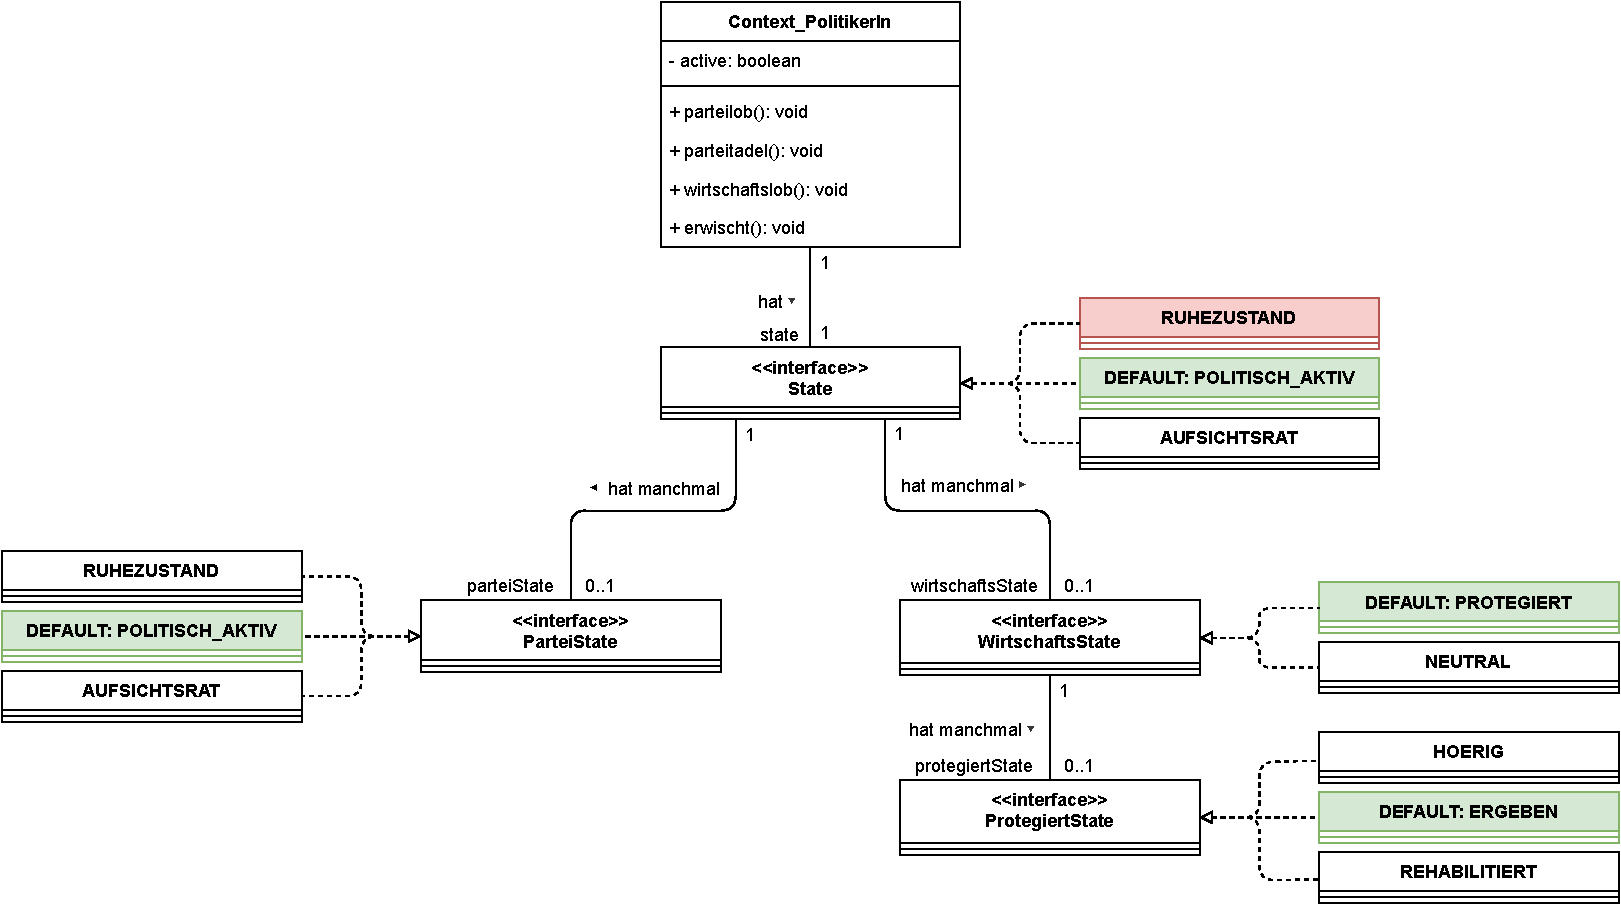
\includegraphics[width=\textwidth]{swt_wende_tim_h10_class_diagram.pdf}
                \caption{\texttt{class\_diagram}}
            \end{figure}
            
            \begin{itemize}
                \item Die im Klassendiagramm dargestellten Interfaces sind offensichtlich Implementierungen dieser.
                    Daher gehören die durch Rollen implizit gegebenen Attribute auch zu den Interfaces
                \item Die \textcolor{green}{grün} dargestellten Klassen sind die default Klassen
                \item Die \textcolor{red}{rot} dargestellten Klassen sind Endzustände
            \end{itemize}

            \newpage
            Hier die vollständige Version aus Visual Paradigm:

            \begin{figure}[ht]
                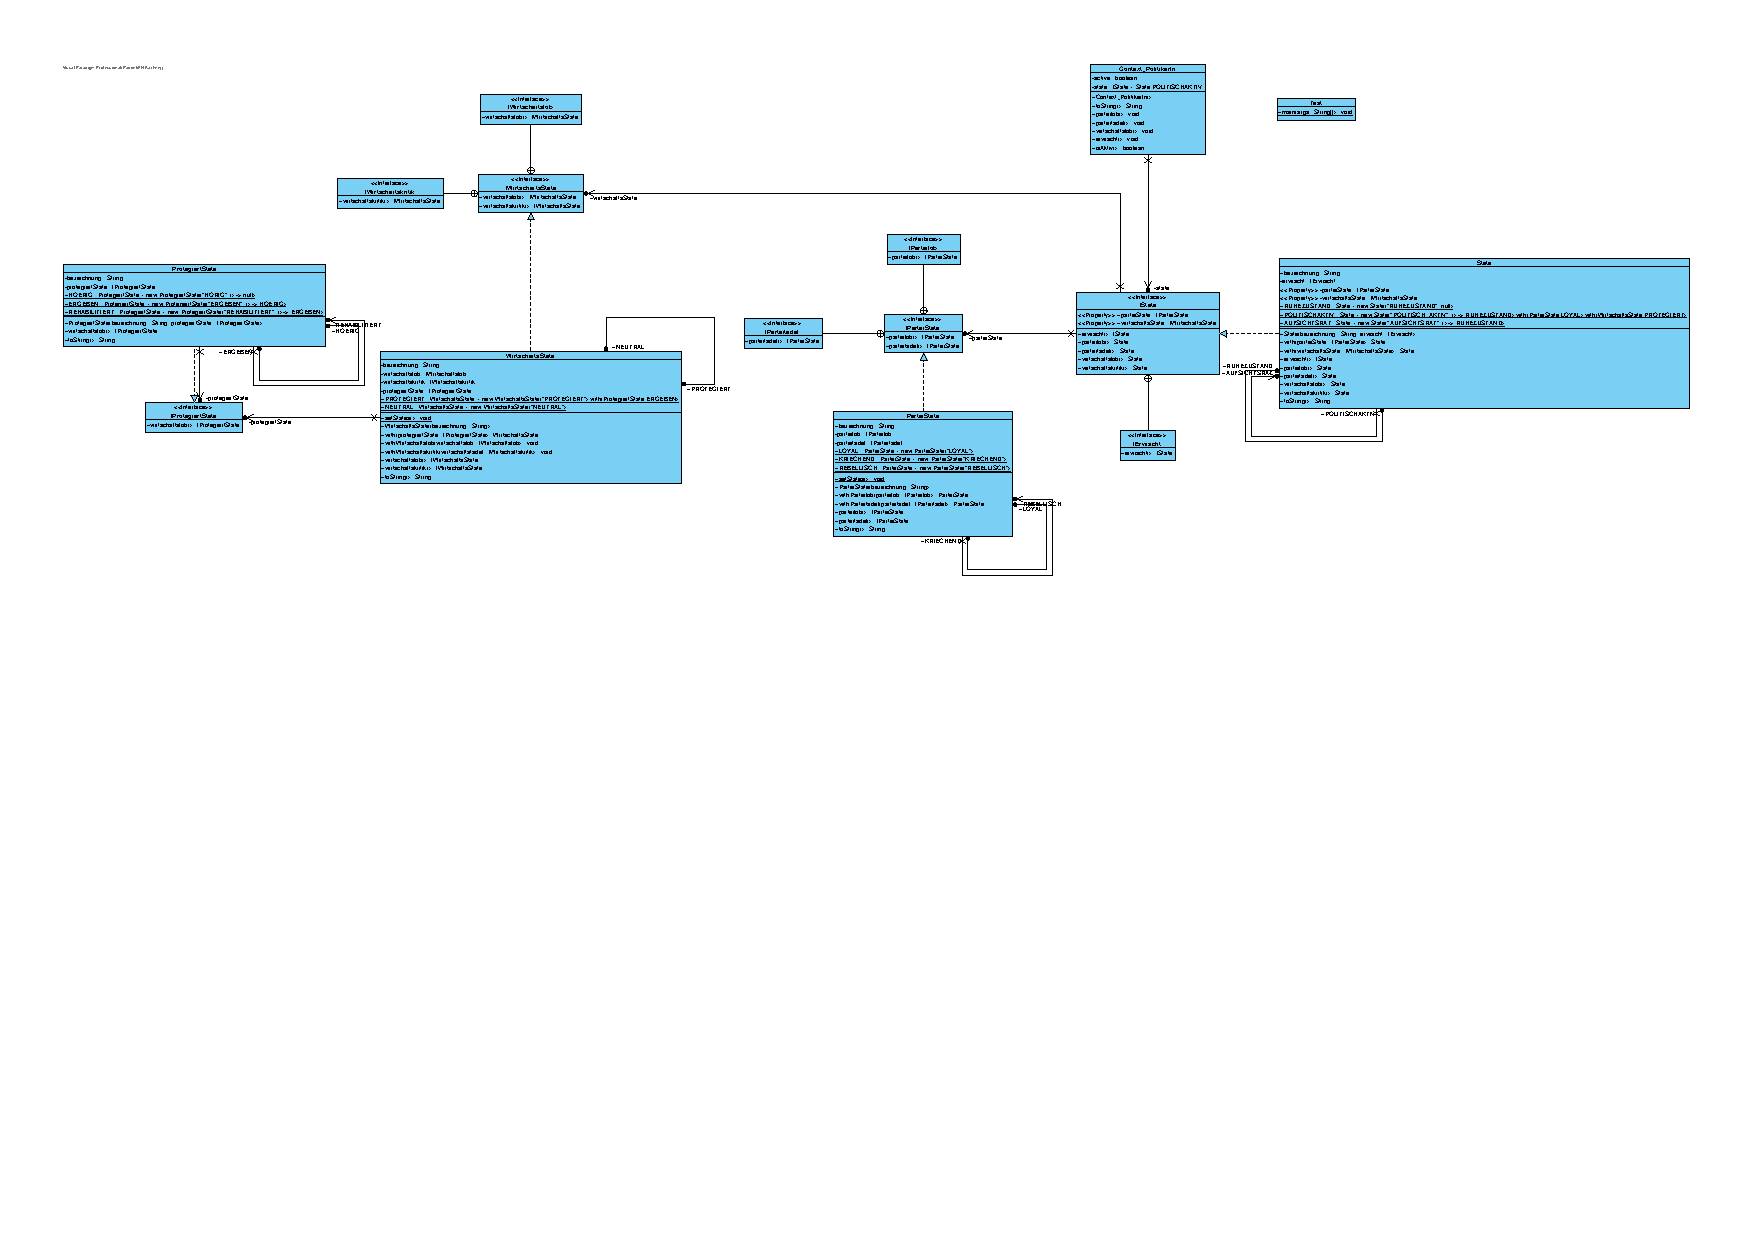
\includegraphics[trim=0cm 10cm 0cm 0cm, width=\textwidth]{swt_wende_tim_h10_class_diagram_vp.pdf}
                \caption{\texttt{class\_diagram\_vp}}
            \end{figure}

            Hier der gegebene Zustandsautomat dazu:\\
            (Wer auch immer den Pfeil von \texttt{hörig} zu \texttt{Aufsichtsrat} erstellt hat :/ )

            \begin{figure}[ht]
                \centering
                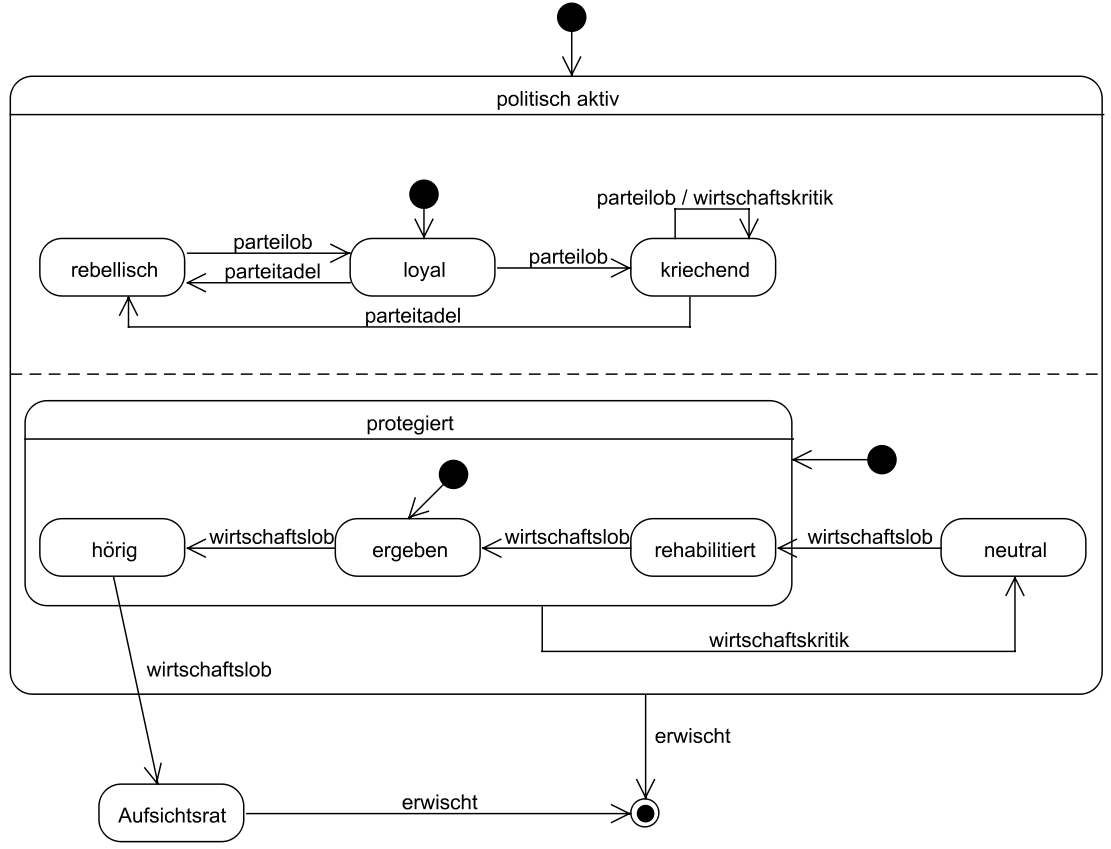
\includegraphics[width=0.75\textwidth]{politiker_zustandsautomat.png}
                \caption{\texttt{politiker\_zustandsautomat}}
            \end{figure}

            \newpage
            Hier die leicht veränderte Steuerung:

            \inputminted{java}{Steuerung.java}

            \newpage
            Und hier meine Testklasse:
            \inputminted{java}{Test.java}

            Auch in dieser Hausaufgabe entfallen alle weiteren Klassen, jedoch hier noch ein Paar Kommentare:

            \begin{itemize}
                \item Die Klassen mit dem Präfix \texttt{I} sind offensichtlich Interfaces.
                    So weit, so bekannt, jedoch sind die Klassen ohne das eben besagte \texttt{I} Gerüst Klassen, welche genutzt werden, um nicht jede Klasse einzeln implementieren zu müssen.
                    So nutze ich beispielsweise \texttt{State} drei mal (bzw. drei Objekte der Klasse \texttt{State}) anstatt die Klassen \texttt{RUHEZUSTAND}, \texttt{POLITISCHAKTIV}, \texttt{AUFSICHTSRAT} \ldots
                    Diese sind dann als static Attribute in den Klassen zu finden:

                    \begin{minted}{java}
public static final State RUHEZUSTAND = new State("RUHEZUSTAND", null);
public static final State POLITISCHAKTIV = new State("POLITISCH_AKTIV", () -> RUHEZUSTAND)
    .with(ParteiState.LOYAL).with(WirtschaftsState.PROTEGIERT);
public static final State AUFSICHTSRAT = new State("AUFSICHTSRAT", () -> RUHEZUSTAND);
                    \end{minted}

                    Selbes Spiel wie in der letzten Hausaufgabe: Da die Objekte \texttt{final} sind, können diese \texttt{public sein}.\\
                    Wenn man mit mehreren PolitikerInnen parallel arbeitet, muss man copy ctors für diese DEFAULT Attribute nutzen.
                    Da diese jedoch dann in einem anderen Kontext existieren würden bzw dieser Fall gar nicht vorgesehen ist, habe ich diese nicht implementiert.

                \item Ich bin davon ausgegangen, dass ein/e PolitikerIn nicht in mehreren Zuständen sein kann, da die initial Zustände in POLITISCH\_AKTIV keine parallelen Aubläufe darstellen.
                    Demensprechend habe ich die Zustände wie \href{http://www.modeler.org.cn/tool/ToolsEA/UserGuide/model_simulation/multi-threading_-_concurrent_s.html}{hier} zu sehen implementiert.
                    Sollte der Zustand bei \texttt{ii. POLITISCH\_AKTIV KRIECHEND AUFSICHTSRAT} sein, müsste man mehrere Zustände bei dem/der PolitikerIn ermöglichen.
                    Dies ist natürlich dann nicht realitätsnah, nicht wahr liebe (leider) nicht ganz fiktive CDU Politiker.

                \item Das Interface \texttt{ParteiState} könne von \texttt{Parteilob} erben.
                    Von dort aus könne \texttt{State} weiter die Methoden erben.
                    Dies würde Code-dopplung verhindern und dank Javadoc die Klassen leesbarer machen.
                    Dies hat jedoch nicht auf Anhieb funktioniert und Java wehrt sich irgendwie dagegen.
                    Apropos: Auf Javadoc musste leider aus Zeit-Gründen verzichtet werden.

                \item Ich habe mal für jede Methode ein eigenes Interface erstellt, dies hilft mir beim Erstellen der DEFAULT Klassen.
                    Sollte dies nicht gewollt sein, müsste man eigene (private inner) Klassen erstellen.
                    Mehr dazu in der Ersten Anmerkung. 
            \end{itemize}
            
            Eine gute Erklärung zum State-Pattern ist \href{https://www.philipphauer.de/study/se/design-pattern/state.php}{hier} zu finden.

            P.S. Machen Sie sich Gedanken darüber, wie eine Aktion wie z.B. \gqq{wirtschaftskritik} aus dem Unterzustand \gqq{politisch aktiv} an protegiert weitergeleitet werden kann:

            In meiner Lösung; gar nicht.
            Man könnte den \texttt{State} durch die verschiedenen Methoden durchreichen, oder den Kontekt \texttt{public} machen.
            Alternativ reagiert man auf die resultierenden Umstände, wie in meinem Code.
    \end{enumerate}
\end{document}